\documentclass[9pt,twocolumn]{pnas-new}
\templatetype{pnasresearcharticle}
\setboolean{displaywatermark}{false}

\usepackage{amsmath,amssymb}
\usepackage{booktabs}
\usepackage{graphicx}
\usepackage{float}
\usepackage{placeins}

\graphicspath{{figures/}}
% Auto-generated by scripts/build_causal_package.py
\newcommand{\TotalPapers}{5,922}
\newcommand{\TotalReviews}{20,427}
\newcommand{\AcceptedPapers}{2,159}
\newcommand{\RejectedPapers}{3,763}
\newcommand{\OverallAcceptancePct}{36.5}
\newcommand{\SentimentAcceptMean}{0.749}
\newcommand{\SentimentRejectMean}{0.580}
\newcommand{\PolitenessAcceptMean}{0.493}
\newcommand{\PolitenessRejectMean}{0.413}
\newcommand{\ToxicityAcceptMean}{0.001}
\newcommand{\ToxicityRejectMean}{0.001}
\newcommand{\ConstructivenessAcceptMean}{1.221}
\newcommand{\ConstructivenessRejectMean}{1.211}
\newcommand{\MeanScoreAccept}{6.56}
\newcommand{\MeanScoreReject}{4.55}
\newcommand{\ReviewLengthAccept}{363.9}
\newcommand{\ReviewLengthReject}{371.2}
\newcommand{\PaperSentimentAME}{-0.002}
\newcommand{\PaperSentimentAMECI}{[-0.017, 0.014]}
\newcommand{\ReviewSentimentAME}{0.195}
\newcommand{\ReviewSentimentAMECI}{[0.181, 0.211]}
\newcommand{\ReviewPolitenessAME}{0.048}
\newcommand{\ReviewPolitenessAMECI}{[0.036, 0.059]}
\newcommand{\ReviewConstructivenessAME}{0.011}
\newcommand{\ReviewConstructivenessAMECI}{[0.002, 0.018]}
\newcommand{\PredProbLowSent}{0.366}
\newcommand{\PredProbHighSent}{0.364}
\newcommand{\BaselineAUCMin}{0.955}
\newcommand{\BaselineAUCMax}{0.963}
\newcommand{\MaxAbsDeltaAUC}{0.0005}
\newcommand{\YearSentimentDiffMin}{0.123}
\newcommand{\YearSentimentDiffMax}{0.189}
\newcommand{\YearPolitenessDiffMin}{0.059}
\newcommand{\YearPolitenessDiffMax}{0.106}
\newcommand{\BorderlinePapers}{1,878}
\newcommand{\MatchedPairs}{695}
\newcommand{\PSMATT}{0.004}
\newcommand{\PSMATTCI}{[-0.037, 0.043]}
\newcommand{\PSMNarrowATT}{0.009}
\newcommand{\PSMNarrowATTCI}{[-0.040, 0.054]}
\newcommand{\PSMWideATT}{0.011}
\newcommand{\PSMWideATTCI}{[-0.027, 0.052]}
\newcommand{\PSMRobustATT}{-0.054}
\newcommand{\PSMRobustATTCI}{[-0.109, 0.000]}
\newcommand{\BalanceStatus}{passed}
\newcommand{\ClusterCount}{12}
\newcommand{\HeteroYearMin}{-0.039}
\newcommand{\HeteroYearMax}{0.024}
\newcommand{\HeteroDisagreementMin}{-0.021}
\newcommand{\HeteroDisagreementMax}{0.008}


\title{Review language tracks acceptance but adds little predictive value in AI peer review}

\author[a,1]{Author Placeholder1}
\author[b,2]{Author Placeholder2}

\affil[a]{Affiliation placeholder}
\affil[b]{Affiliation placeholder}

\leadauthor{Placeholder}
\significancestatement{Peer-review archives preserve more than ratings and final decisions: they also preserve the language through which scientific judgments are rendered. Reconstructing the raw ICLR archive shows that accepted papers receive more positive review language and that review-level sentiment closely aligns with favorable recommendations. Yet once scores, disagreement, confidence, and manuscript-side controls are observed, language contributes little additional predictive value for final acceptance. The result reframes review text as an evaluative trace that is socially meaningful and institutionally important, while cautioning against claims that language alone is a powerful hidden driver of scientific selection.}
\authorcontributions{Author contributions placeholder: this draft should be updated with the final contribution statement before submission.}
\authordeclaration{The authors declare no competing interest in this draft.}
\equalauthors{Author placeholder note: authorship ordering and equal-contribution statements remain to be finalized.}
\correspondingauthor{Correspondence should be addressed to the project team after author metadata are finalized.}
\keywords{peer review | computational social science | OpenReview | research evaluation | machine learning}

\begin{abstract}
Peer review is both a scoring system and a language-mediated institution, yet large-scale studies of scientific evaluation often treat review text as secondary to formal ratings. We reconstruct the raw ICLR OpenReview archive and harmonize \TotalPapers{} submissions and \TotalReviews{} reviews from 2018 to 2023 to examine how review language relates to recommendation and final acceptance. Accepted papers receive more positive paper-level review language than rejected papers (\SentimentAcceptMean{} versus \SentimentRejectMean{}), along with slightly higher politeness (\PolitenessAcceptMean{} versus \PolitenessRejectMean{}), negligible toxicity differences (\ToxicityAcceptMean{} versus \ToxicityRejectMean{}), and only weak constructiveness differences (\ConstructivenessAcceptMean{} versus \ConstructivenessRejectMean{}). At the review level, sentiment strongly aligns with favorable recommendations (average marginal effect \ReviewSentimentAME{}, 95\% CI \ReviewSentimentAMECI{}). At the paper level, however, that association largely attenuates once mean score, disagreement, confidence, review structure, manuscript-side metadata, year fixed effects, and topic-cluster fixed effects are included: predicted acceptance moves only from \PredProbLowSent{} to \PredProbHighSent{} across the observed sentiment range. The descriptive sentiment gap remains positive in every conference year, ranging from \YearSentimentDiffMin{} to \YearSentimentDiffMax{}, but leave-one-year-out models gain at most \MaxAbsDeltaAUC{} AUC from adding language, and a matched borderline comparison of \BorderlinePapers{} papers yields a primary estimate of \PSMATT{} (95\% CI \PSMATTCI{}). Review language therefore tracks evaluative judgment and final outcomes, yet adds little independent predictive value once the broader review profile is observed.
\end{abstract}

\dates{Compiled \today}
\doi{DOI placeholder}

\begin{document}
\maketitle
\thispagestyle{firststyle}
\pagestyle{plain}

Scientific evaluation is rendered through language before it is reduced to a binary decision. Reviewers praise, hedge, criticize, and justify, turning local judgments into text that authors, editors, and later observers can inspect \cite{walker2015peerreview,tennant2017innovations}. Open peer-review platforms make that communicative layer unusually visible because they preserve the documentary surface of evaluation rather than only the terminal verdict \cite{openreview2026iclr}. For computational social science, such archives are valuable precisely because they expose scientific selection as a social process expressed in words as well as numbers \cite{lazer2009computational}. More broadly, recent work on scientific language suggests that wording can shape how merit is signaled and perceived, making peer-review discourse a substantive object of study rather than editorial residue \cite{stavrova2025promotional}.

That visibility creates an empirical puzzle. Review language may matter because it frames evidence, emphasizes strengths, softens criticism, and makes recommendations legible. But it is also easy to overread. More positive wording may simply accompany stronger papers; politeness may coexist with rejection in professional settings; toxicity may be too rare to structure outcomes; and constructive critique may intensify exactly when reviewers are unconvinced. Because text and scores are co-produced in the same evaluative encounter, observational archives are well suited to documenting alignment between language and outcomes but are less suited to claims that wording itself independently drives acceptance.

We examine that puzzle in ICLR, a leading AI conference whose OpenReview records preserve review texts, reviewer recommendations, and final decisions. Using the raw 2018--2023 archive, we ask whether accepted and rejected papers are described differently, whether any paper-level language association remains once score-based evaluation profiles are observed, and whether those patterns are stable across yearly cohorts and in the score-overlap region where accepted and rejected papers are most comparable. The design therefore moves deliberately from broad descriptive evidence to more restrictive comparisons.

The analysis combines full-archive descriptive comparisons, review-level models of recommendation, paper-level fixed-effects models of final acceptance, year-by-year and disagreement-based heterogeneity analyses, coarse score-bin bridge diagnostics, and a matched borderline comparison centered on the 35th--65th score percentiles. Each layer answers a different version of the same question. Descriptive comparisons show how successful and unsuccessful submissions are discussed. Conditioned paper-level models ask whether language retains measurable acceptance association once stronger evaluation proxies are already known. Matched borderline comparisons ask whether any sentiment-linked difference survives among papers that are more comparable on observed features.

The contribution is deliberately cautious. We do not treat review text as a hidden substitute for formal recommendation fields, and we do not present matching as clean causal identification. Instead, we show that review language is best understood as an evaluative trace. Accepted papers are described differently, and favorable recommendations are voiced differently, but most of that difference travels with the broader score structure through which scientific judgment becomes visible.

\section{Results}

\subsection{Raw-archive reconstruction and analytic layers}

The paper rests on a rebuilt raw archive rather than on previously aggregated outputs. Harmonizing year-specific OpenReview fields yields \TotalPapers{} paper submissions and \TotalReviews{} review texts from ICLR 2018--2023, with one review-level table and one paper-level table as the canonical analytic interfaces. Across the six conference cohorts, the overall acceptance rate is \OverallAcceptancePct\%, ranging from 31.3\% in 2020 to 40.7\% in 2023. Appendix Tables~\ref{tab:app:harmonization} and~\ref{tab:app:fieldmap} document the year-specific parsing choices that map changing archive schemas into a common review text, score or recommendation, confidence, and decision structure.

The empirical design then proceeds in two layers. The first uses the full archive to characterize both raw descriptive separation and conditional associations through paper-level comparisons, review-level models of positive recommendation, paper-level fixed-effects models of final acceptance, year-by-year contrasts, subgroup heterogeneity analyses, and held-out predictive diagnostics. The second is narrower and more conservative: it isolates the central score region, where accepted and rejected papers plausibly overlap, and asks whether higher review sentiment still corresponds to a meaningfully different acceptance rate once observable evaluation profiles are aligned.

These design choices are motivated by the archive itself. Appendix Figure~\ref{fig:app:measurement} reports parser completeness, review-count distributions, review-length distributions, and metadata coverage by year; the largest year-specific break is confidence parsing in 2020, where the export does not preserve a directly comparable field. Appendix Figure~\ref{fig:app:correlations} shows that language features co-move with score proxies and review-structure variables rather than floating independently of them. Those diagnostics matter because they define the evidentiary boundary of the study: the archive can support strong descriptive and observational claims, but only with explicit acknowledgment of field drift, selective missingness, and noisy topic proxies.

\begin{figure*}[t]
\centering
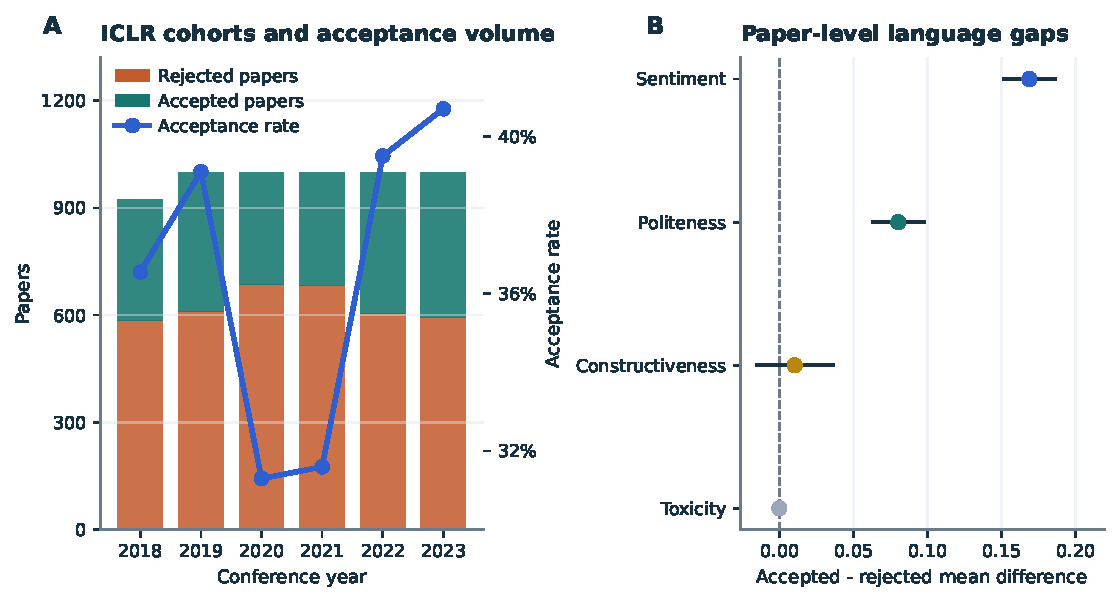
\includegraphics[width=\textwidth]{figure1_overview.pdf}
\caption{\textbf{Archive overview and first-pass language differences in ICLR peer review.} \textbf{A}, Yearly paper counts and acceptance rates in the rebuilt ICLR 2018--2023 archive. The panel situates the analysis in the institutional scale of the conference: after the smaller 2018 cohort, submission volume is broadly high and acceptance rates move within a relatively narrow band, indicating that the main descriptive patterns are not driven by a single unusual year. \textbf{B}, Accepted-minus-rejected mean differences in the four paper-level language measures, with 95\% confidence intervals. The descriptive separation is concentrated in sentiment and, more modestly, politeness, whereas constructiveness differs only slightly and toxicity is substantively near zero. Taken together, the two panels establish the paper's first empirical claim: accepted papers are discussed more positively, but not simply in a uniformly friendlier way on every language dimension.}
\label{fig:overview}
\end{figure*}

\subsection{Accepted papers receive more positive review language, and review-level sentiment aligns with recommendation}

Accepted papers are described in more positive terms. At the paper level, mean sentiment is higher for accepted than rejected submissions (\SentimentAcceptMean{} versus \SentimentRejectMean{}), and mean politeness is also modestly higher (\PolitenessAcceptMean{} versus \PolitenessRejectMean{}). By contrast, toxicity is essentially indistinguishable across outcomes (\ToxicityAcceptMean{} versus \ToxicityRejectMean{}), and constructiveness differs only weakly (\ConstructivenessAcceptMean{} versus \ConstructivenessRejectMean{}). Figure~\ref{fig:overview} makes the pattern visible: the main descriptive separation lies in evaluative valence rather than in broad shifts toward hostility or universally softer language.

That descriptive separation coexists with a much larger formal evaluation gap. Accepted papers have substantially higher mean reviewer scores than rejected papers (\MeanScoreAccept{} versus \MeanScoreReject{}), whereas average review length is broadly similar across outcomes (\ReviewLengthAccept{} versus \ReviewLengthReject{} words). The key point is not that language substitutes for score, but that the score gap is accompanied by a systematic change in how papers are verbally framed. In a professional venue where reviewers are expected to remain civil, positivity appears to be the channel through which evaluation differences become most legible in text.

The review-level model sharpens that interpretation. In year- and topic-adjusted specifications, higher review sentiment is associated with a markedly greater probability that an individual review carries a positive recommendation (average marginal effect \ReviewSentimentAME{}, 95\% CI \ReviewSentimentAMECI{}; Appendix Table~\ref{tab:app:reviewame}). Secondary tone dimensions are much smaller: politeness is positively associated with recommendation, constructiveness is modestly positive, and toxicity is imprecisely negative. This is the clearest point in the paper at which language and recommendation move together. At the level of individual reviews, more positive wording is closely aligned with a more favorable reviewer stance, even if that alignment should not be interpreted as a causal language effect.

The descriptive and review-level findings therefore establish the paper's first result. Review comments matter in the documentary sense that successful and unsuccessful submissions are discussed differently, and favorable recommendations are voiced differently. The remaining question is whether that language still carries much paper-level acceptance association once the broader evaluation profile is already visible.

\begin{figure*}[t]
\centering
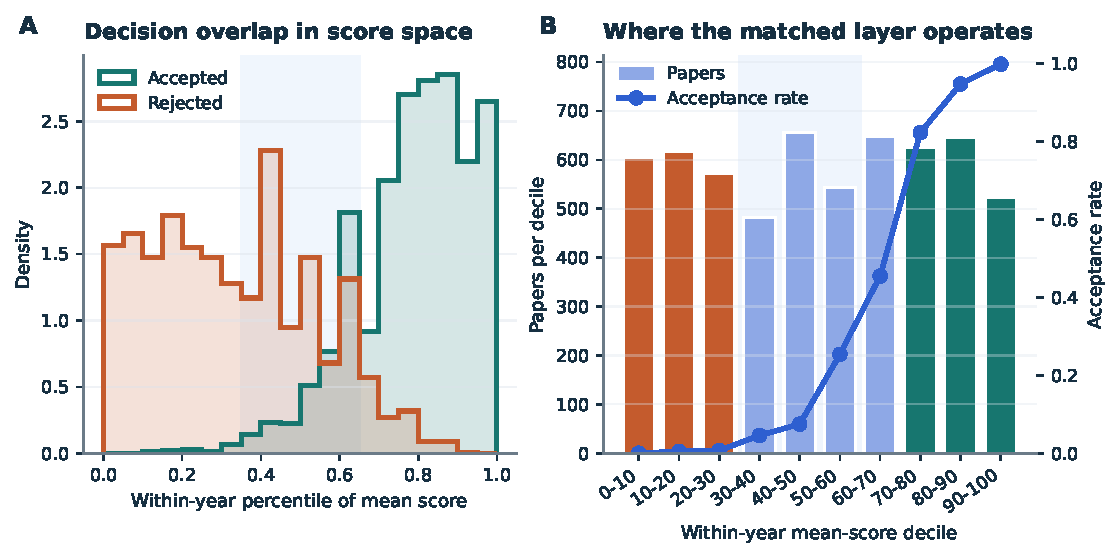
\includegraphics[width=\textwidth]{figure1_design_motivation.pdf}
\caption{\textbf{Score overlap motivates the narrower matched layer.} \textbf{A}, Distributions of within-year mean-score percentiles for accepted and rejected papers. Overlap between the two outcome groups is concentrated in the middle of the score distribution rather than at the extremes, where decisions are already close to deterministic. \textbf{B}, Paper counts and acceptance rates by within-year mean-score decile. The shaded middle band marks the 35th--65th percentile window used for the primary borderline design, yielding \BorderlinePapers{} papers. The figure provides the design logic for the matched analysis: if any sentiment-linked acceptance contrast is going to survive after stronger alignment on observed evaluation profiles, it should be sought in the central score region rather than among papers whose outcomes were already nearly fixed by score.}
\label{fig:design}
\end{figure*}

\subsection{Once score-based evaluation profiles are included, paper-level sentiment adds little independent leverage}

Conditioning on the broader evaluation profile largely flattens the paper-level sentiment gradient. The paper-level acceptance model includes mean sentiment as the focal predictor while conditioning on mean score, score disagreement, reviewer confidence, number of reviews, mean review length, title length, abstract length, keyword count, year fixed effects, and keyword-based topic-cluster fixed effects. In that specification, the average marginal effect of paper-level sentiment is \PaperSentimentAME{} with a 95\% confidence interval of \PaperSentimentAMECI{} (Appendix Table~\ref{tab:app:paperame}).

Figure~\ref{fig:papermargins} converts that estimate into model-implied probabilities. Across the observed sentiment range, predicted acceptance changes only from \PredProbLowSent{} to \PredProbHighSent{}. The fitted line is therefore nearly flat relative to the raw outcome separation. Mean score remains the dominant organizing variable in the model, and once that broader evaluation profile is already in view, paper-level sentiment contributes little additional acceptance separation.

The contrast between the two panels is the substantive point. Panel A shows how little conditional movement remains after controls, whereas Panel B preserves the raw accepted-versus-rejected sentiment separation in the underlying data. Read together, they show that review language is informative descriptively but weak as an independent paper-level discriminator once stronger proxies for reviewer evaluation are included. That contrast also helps reconcile the review-level and paper-level results: sentiment is tightly linked to how reviewers express their recommendations, but the aggregate decision is already so well organized by scores and related review structure that little additional paper-level leverage remains for language alone.

Appendix-only predictive diagnostics tell the same story in a complementary register. Leave-one-year-out baseline models that use scores and manuscript-side controls already reach AUCs between \BaselineAUCMin{} and \BaselineAUCMax{} (Appendix Table~\ref{tab:app:prediction}; Appendix Figure~\ref{fig:app:prediction}). Adding paper-level language features changes held-out AUC by at most \MaxAbsDeltaAUC{}. The archive therefore offers little support for the stronger claim that review text contains a large hidden acceptance signal not already reflected in formal evaluation variables.

That predictive near-null is substantively useful because it clarifies what review text is and is not doing in this setting. In discussions of automated triage or text-based editorial support, it is tempting to imagine review prose as a rich shadow predictor that can outperform more structured fields. The present archive does not support that interpretation. Once score, disagreement, confidence, and basic manuscript-side metadata are known, language adds very little held-out discrimination. Its value appears to lie more in interpretation, auditing, and justification than in providing a large extra predictive shortcut.

A coarse bridge analysis helps connect the descriptive and matched layers. Appendix Figure~\ref{fig:app:bridge} and Appendix Table~\ref{tab:app:bridge} show that once papers are compared within year-specific score deciles, the full-sample sentiment gap attenuates sharply in the middle of the score distribution, which is exactly where accepted and rejected papers overlap most plausibly. The dramatic gaps at the top and bottom deciles are less informative about incremental language differences because acceptance is already close to deterministic in those regions. This bridge helps explain why both the fixed-effects model and the matched borderline design return near-null residual sentiment associations.

\begin{figure*}[t]
\centering
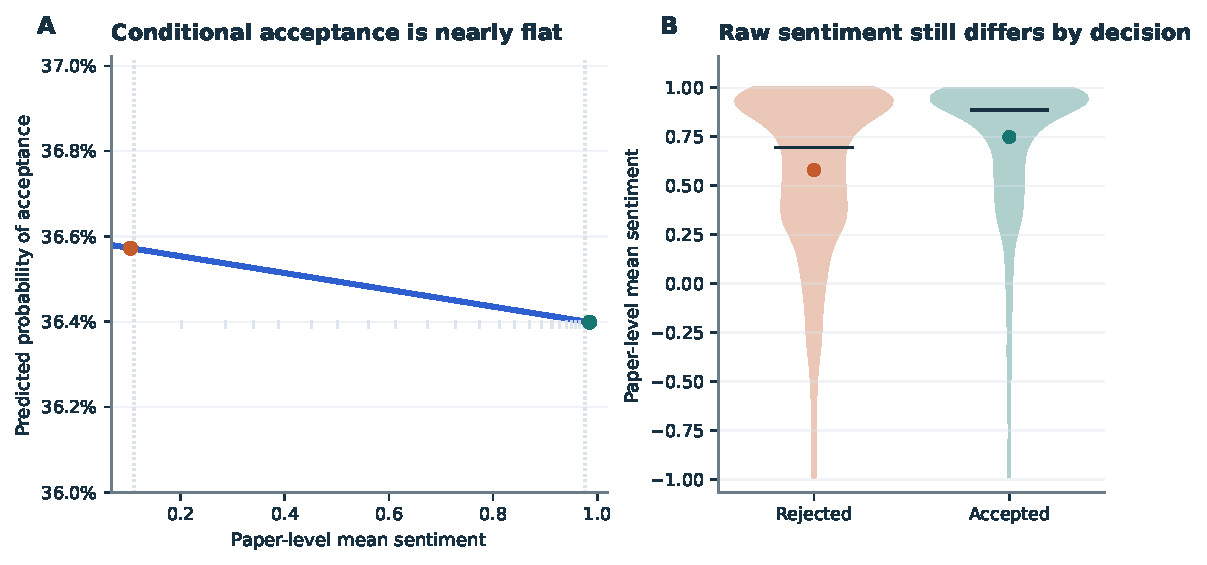
\includegraphics[width=\textwidth]{figure2_paper_fe_margins.pdf}
\caption{\textbf{Raw separation remains visible, but conditional paper-level margins are nearly flat.} \textbf{A}, Model-implied probability of acceptance across the observed paper-level sentiment range after conditioning on mean score, score disagreement, confidence, review volume, review length, manuscript-side controls, year fixed effects, and keyword-based topic-cluster fixed effects. Rug marks show empirical support across the sentiment distribution, and the fitted line moves only from \PredProbLowSent{} at the low end to \PredProbHighSent{} at the high end. \textbf{B}, Raw paper-level sentiment distributions by final decision. The figure is constructed to display the paper's core contrast in a single visual frame: accepted papers are indeed described more positively in the raw data, but once stronger evaluation proxies are included, the remaining paper-level sentiment gradient becomes minimal.}
\label{fig:papermargins}
\end{figure*}

\subsection{Matched borderline comparisons do not support a large additional sentiment-linked acceptance premium}

Restricting the analysis to borderline papers does not restore a large sentiment-linked acceptance premium. Figure~\ref{fig:design} shows why the matched layer is centered on the middle of the score distribution: accepted and rejected papers overlap there far more plausibly than they do at the extremes. We therefore define a within-year borderline region by keeping papers between the 35th and 65th percentiles of the mean-score distribution, yielding \BorderlinePapers{} papers. Within that analytic sample, the matching indicator is above-median versus below-median paper-level sentiment within year. Propensity scores are estimated from mean score, score disagreement, confidence, number of reviews, mean review length, title length, abstract length, keyword count, year, and keyword-based topic-cluster proxies, with exact-year nearest-neighbor matching.

This is the paper's most demanding observational comparison. If the raw descriptive gap reflected a practically large sentiment-linked acceptance difference that survived alignment on observed evaluation profiles, the signal should still be visible in the score-overlap region. Instead, the matched estimate remains small. In the primary borderline design, the matched acceptance difference between higher-sentiment and lower-sentiment papers is \PSMATT{} with a 95\% confidence interval of \PSMATTCI{}.

Figure~\ref{fig:matched} shows both the substantive estimate and the design diagnostics. The primary balance check passes, the matched sample contains \MatchedPairs{} pairs across all six conference years (Appendix Table~\ref{tab:app:matchedcounts}), and standardized mean differences shrink below conventional thresholds after matching. Yet even in that more comparable subset of papers, the estimated acceptance difference remains near zero. The near-null result is therefore informative rather than incidental: it emerges in the part of the archive where a residual paper-level sentiment association has the strongest design-based case to appear.

Sensitivity checks reinforce the same conclusion. Narrowing the score window to the 40th--60th percentile yields \PSMNarrowATT{} (95\% CI \PSMNarrowATTCI{}), widening it to the 30th--70th percentile yields \PSMWideATT{} (95\% CI \PSMWideATTCI{}), and redefining treatment as the top versus bottom sentiment tercile after dropping the middle tercile yields \PSMRobustATT{} (95\% CI \PSMRobustATTCI{}). None of these variants supports a robust, positive, and practically large sentiment-linked acceptance association. The matched layer therefore strengthens the paper's core interpretation rather than softening it.

Appendix Figure~\ref{fig:app:overlap} provides the complementary overlap view by plotting propensity-score distributions before and after matching. Its value is transparency: the near-zero matched estimates are not produced by visibly failed overlap or an obviously poor match. They arise after restricting attention to the region of the archive where high-sentiment and low-sentiment papers are already closest on observed evaluation profiles.

\begin{figure*}[t]
\centering
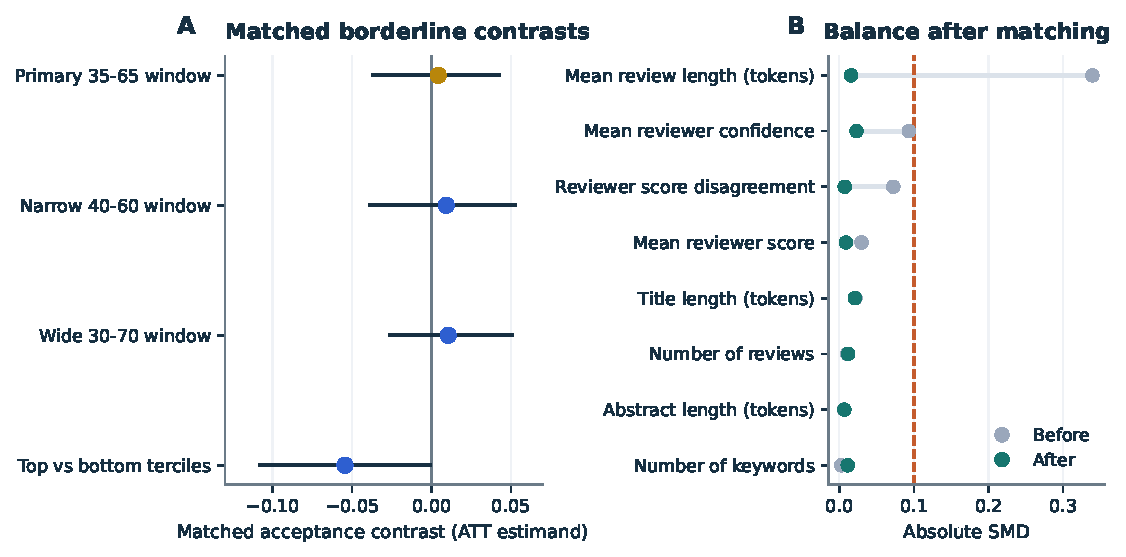
\includegraphics[width=\textwidth]{figure3_matched_effect_balance.pdf}
\caption{\textbf{Matched observational evidence from the borderline layer.} \textbf{A}, Estimated matched acceptance contrast (ATT estimand) for the primary borderline specification and prespecified sensitivity checks. None of the matched specifications yields a clearly positive and practically large sentiment-linked acceptance difference; the primary estimate is \PSMATT{} with a 95\% confidence interval of \PSMATTCI{}. \textbf{B}, Covariate balance diagnostics for the primary matched sample. Absolute standardized mean differences shrink sharply after matching and all core covariates fall below the conventional $|SMD| = 0.10$ benchmark. The figure links design quality to substantive interpretation: the near-zero matched estimates arise in a sample with visibly improved balance, not from a visibly failed match or a trivially nonoverlapping treatment comparison.}
\label{fig:matched}
\end{figure*}

\subsection{Descriptive gaps are stable across years, while conditional heterogeneity remains modest}

The descriptive gap is temporally durable. Accepted papers receive more positive language in every yearly cohort, with sentiment gaps ranging from \YearSentimentDiffMin{} to \YearSentimentDiffMax{} (Appendix Table~\ref{tab:app:yearlygaps}; Appendix Figure~\ref{fig:app:temporal}). Politeness gaps are smaller but also positive in every year, ranging from \YearPolitenessDiffMin{} to \YearPolitenessDiffMax{}. Even as the venue changes in scale, selectivity, and topical composition, the raw accepted-versus-rejected language gap does not reverse direction.

That stability matters because it argues against the descriptive pattern being an artifact of one unusual conference cycle. The six yearly cohorts differ in submission volume, acceptance rates, and review environment, yet accepted papers are still discussed more positively each time. Of all the empirical regularities in the paper, this one is the most institution-like: evaluative tone repeatedly aligns with final success at the descriptive level, even in a rapidly changing AI field.

Conditional heterogeneity is much more muted. Figure~\ref{fig:heterogeneity} shows that the average marginal effect of paper-level sentiment varies only within a narrow band across years and disagreement strata. Year-specific paper-level effects range from \HeteroYearMin{} to \HeteroYearMax{}, and disagreement-specific effects range from \HeteroDisagreementMin{} to \HeteroDisagreementMax{}. Once the model already conditions on scores and related controls, there is no obvious subgroup in which sentiment becomes a large paper-level separator. The disagreement pattern is especially informative because it cuts against the stronger claim that language becomes decisive precisely where formal review signals are most contested.

Topic-cluster heterogeneity points the same way. Appendix Figure~\ref{fig:app:topichetero} and Appendix Table~\ref{tab:app:heterotopic} show movement across keyword-based topical clusters, but not a pattern in which one recognizable subfield displays a consistently large and positive paper-level sentiment association. That reduces the risk that the pooled near-null result is merely averaging together strong topic-specific effects with opposite signs.

The temporal and heterogeneity analyses therefore point in different but compatible directions. Descriptively, the language gap is stable and directionally clear. Conditionally, the remaining paper-level slope is small and does not expand much across year, disagreement, or topic group. Together, those results reinforce the paper's broader interpretation: review language is a stable trace of evaluation, but not a large independent paper-level lever once the rest of the evaluation profile is already observed.

\begin{figure*}[t]
\centering
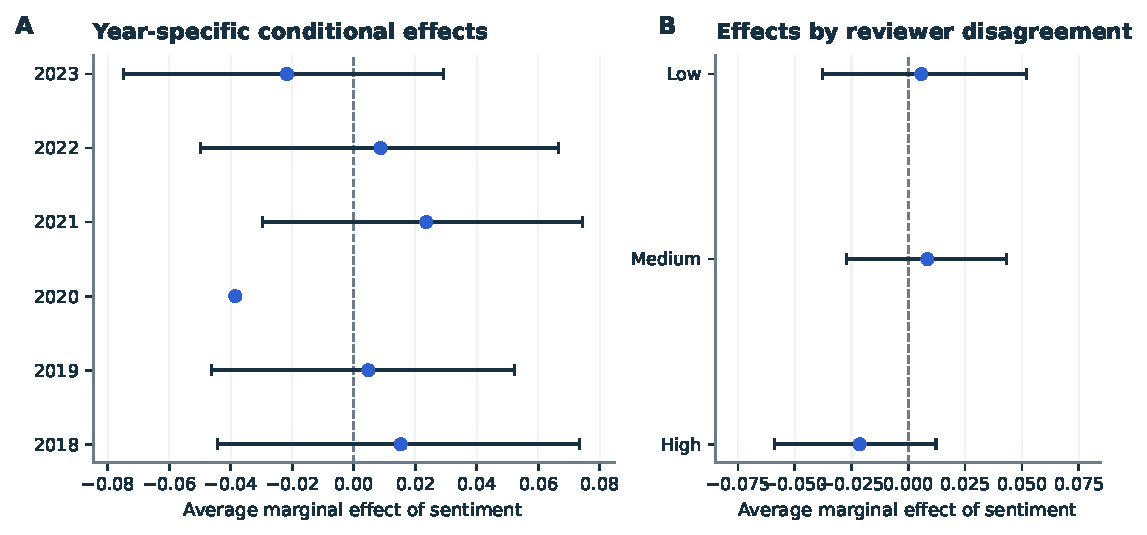
\includegraphics[width=\textwidth]{figure4_heterogeneity_ame.pdf}
\caption{\textbf{Conditional heterogeneity in the paper-level sentiment association.} \textbf{A}, Year-specific average marginal effects of paper-level sentiment from the paper-level model. \textbf{B}, Average marginal effects by disagreement tercile. Across both panels, point estimates remain close to zero relative to the scale of the raw descriptive gaps, and confidence intervals generally straddle small effects. The figure complements the appendix's stable year-by-year descriptive patterns by showing that the conditional paper-level sentiment association does not become large in any obvious conference year or reviewer-disagreement environment.}
\label{fig:heterogeneity}
\end{figure*}

\section{Discussion}

The evidence supports a narrow but robust claim. Review language tracks acceptance, but it adds little independent predictive value once the broader evaluation profile is already visible. Accepted papers are described more positively and somewhat more politely, review-level sentiment strongly aligns with favorable recommendations, and those descriptive gaps are stable across yearly cohorts. Yet paper-level fixed-effects margins are nearly flat, held-out predictive gains are negligible, and matched borderline comparisons remain close to zero.

That pattern is substantively informative because it clarifies how text enters peer review. The archive does not suggest that language is irrelevant. Instead, it suggests that language functions primarily as an evaluative trace: a durable record of how merit, weakness, confidence, and recommendation are phrased. Peer review is not only an allocation mechanism; it is also the institutional setting in which judgments are justified and made legible. A stable descriptive language gap therefore reveals something real about the social grammar of scientific evaluation, even if the same text adds little incremental discrimination beyond scores.

The contrast between review-level and paper-level analyses is especially revealing. At the level of individual reviews, more positive sentiment is closely aligned with a favorable recommendation. At the level of aggregated papers, however, the additional sentiment slope largely disappears once mean score and related controls are included. That divergence suggests that reviewers use language to articulate the same underlying judgments that are also recorded numerically. The text is neither epiphenomenal nor a separate decision engine. It is part of the same evaluative package through which recommendation becomes visible.

The matched borderline layer sharpens that interpretation without converting it into a causal claim. Because language and score are co-produced within the same review round, matching cannot identify an intervention-like effect of wording alone. But it can ask a harder observational question: among papers that look similar on observed evaluation profiles and lie in the region of greatest score overlap, does a large sentiment-linked acceptance contrast remain? The answer is largely no. That is why the matched evidence matters. It does not overturn the descriptive finding; it shows that the descriptive gap rarely translates into a large residual paper-level advantage once like is compared with like.

This interpretation has broader implications for peer-review governance and for computational social science more generally. Open-review platforms preserve the verbal record of evaluation, and that record should not be treated as dispensable simply because it adds little extra AUC after scores are known. Text remains important for transparency, accountability, and interpretability. It is where reviewers qualify praise, phrase uncertainty, and justify criticism. At the same time, the weak conditional paper-level and matched results caution against overstating the promise of text-only ranking systems or language-based acceptance prediction. In this archive, the most defensible value of review language is analytic and institutional: it helps audit evaluative style, identify mismatches between tone and recommendation, and document how decisions are communicated.

Several limitations frame that conclusion. First, the language measures are intentionally transparent and lightweight; they enable an auditable workflow but do not exhaust the semantic richness of review text. Second, manuscript-side controls are limited to local metadata rather than full-paper content in this rebuild. Third, language and scores are generated within the same evaluation process, which is why both the full-archive and matched layers are interpreted in associational rather than causal terms. Fourth, stable official area or track labels are not available in a form that can be harmonized cleanly across all six years, so topic controls rely on keyword-based clusters rather than formal research-area assignments. Finally, the paper is confined to ICLR; replication across other open peer-review venues remains an important next step.

Within those bounds, the main conclusion is straightforward. Review comments matter descriptively and interpretively because they reveal how acceptance and recommendation are linguistically expressed. But they matter much less as an independent paper-level separator once stronger evaluation proxies are already available. For this archive, review language is best understood as part of the observable surface of scientific judgment, not as a hidden standalone driver of selection.

\matmethods{%
\textbf{Data source and harmonization.} The dataset comes from OpenReview, using the ICLR group page (\texttt{https://openreview.net/group?id=ICLR.cc}) and the OpenReview API, and covers conference years 2018--2023 \cite{openreview2026iclr}. We reconstruct the archive directly from year-specific records and harmonize changing field names for review text, score or recommendation, reviewer confidence, and final decision. The resulting package contains a review-level table with one row per review and a paper-level table with one row per submission. Parse-success flags are retained for key fields so that archive completeness can be audited directly.\par
\textbf{Measures.} Sentiment is measured at the review level with VADER and then averaged within paper \cite{hutto2014vader}. The rebuild also retains three transparent secondary tone measures based on marker dictionaries: a politeness index grounded in prior politeness-feature work \cite{danescu2013politeness,chang2020convokit}, a toxicity index based on explicit lexical markers \cite{basile2019hurtlex}, and a constructiveness index designed to capture actionable critical language. These measures are used descriptively and as secondary covariates rather than as the main headline predictors. The paper-level table also stores mean reviewer score, score standard deviation, mean reviewer confidence where available, number of reviews, average review length, title length, abstract length, keyword count, and final accept/reject status.\par
\textbf{Observational layer.} The review-level model predicts whether an individual review gives a positive recommendation, defined as a parsed score or recommendation of at least 6, from review-level sentiment and controls plus year and topic fixed effects. Standard errors are clustered by paper/forum to account for multiple reviews per submission. The paper-level model predicts final acceptance from paper-level mean sentiment, secondary language measures, score, disagreement, confidence, review volume, review length, manuscript-side controls, and year and topic fixed effects. Uncertainty is estimated with clustered covariance at the year level when feasible and robust covariance otherwise. We summarize the paper-level sentiment relationship primarily through marginal predicted probabilities and average marginal effects rather than raw coefficients alone. Cross-year predictive diagnostics train on five conference years and evaluate on the held-out sixth year, comparing a baseline with score and manuscript controls against an extended model that also includes paper-level language features.\par
\textbf{Stability and heterogeneity.} Year-specific descriptive gaps are computed as accepted-minus-rejected differences in paper-level means within each conference year, with standard two-sample confidence intervals. We also estimate year-specific and disagreement-specific paper-level average marginal effects of sentiment using the same observational specification, adapting fixed effects where necessary within subgroups. These analyses are interpreted as heterogeneity diagnostics rather than as evidence of invariant underlying mechanisms.\par
\textbf{Topic proxies.} Because the raw export does not provide a stable official area label that is directly comparable across all years, topic adjustment relies on keyword-based cluster proxies rather than formal tracks. Cleaned author keywords are vectorized with TF--IDF and grouped into deterministic clusters via k-means. These clusters are used as noisy topic controls in both the observational and matching layers rather than as claims about true research areas.\par
\textbf{Matched borderline layer.} The primary matched design keeps papers whose within-year mean-score percentile falls between the 35th and 65th percentiles, producing the borderline analytic sample. A binary high-versus-low sentiment indicator is then defined within year after standardizing sentiment inside that sample. Propensity scores are estimated with exact matching on year and nearest-neighbor matching on the logit propensity score, using a 0.1-standard-deviation caliper and covariates for topic cluster, mean score, score disagreement, confidence, review count, mean review length, title length, abstract length, and keyword count \cite{rosenbaum1983central,austin2009balance}. We report matched high-versus-low sentiment contrasts, standardized mean differences before and after matching, matched-pair counts by year, and bootstrap confidence intervals for the primary and sensitivity specifications. The estimator is used as an observational comparison device rather than as evidence of clean causal identification.\par
\textbf{Interpretation.} All results are interpreted conservatively. Review language and reviewer scores are generated within the same evaluative process, so neither the full-archive observational layer nor the matched borderline layer identifies a clean treatment that temporally precedes the outcome. The manuscript therefore uses the language of association, alignment, stability, and matched observational evidence rather than causal determination. Claims about official areas or tracks are explicitly excluded because consistent labels are unavailable in the harmonized archive.%
}

\showmatmethods

\section*{Data Availability}

The data, code, figures, and derived outputs for this study will be made available through the project GitHub repository. The underlying review records come from OpenReview, using the ICLR group page and the OpenReview API.

\bibliography{references}

\FloatBarrier
\onecolumn
\appendix
\renewcommand{\thetable}{A\arabic{table}}
\setcounter{table}{0}
\renewcommand{\thefigure}{A\arabic{figure}}
\setcounter{figure}{0}
\section*{Appendix: Measurement and Data Validation}
This appendix extends the main text with report-style tables and diagnostic figures covering raw-archive parsing, measurement completeness, bridge analyses between descriptive and matched layers, and legacy diagnostics from the earlier derived-table workflow.

\begin{figure}[!htbp]
\centering
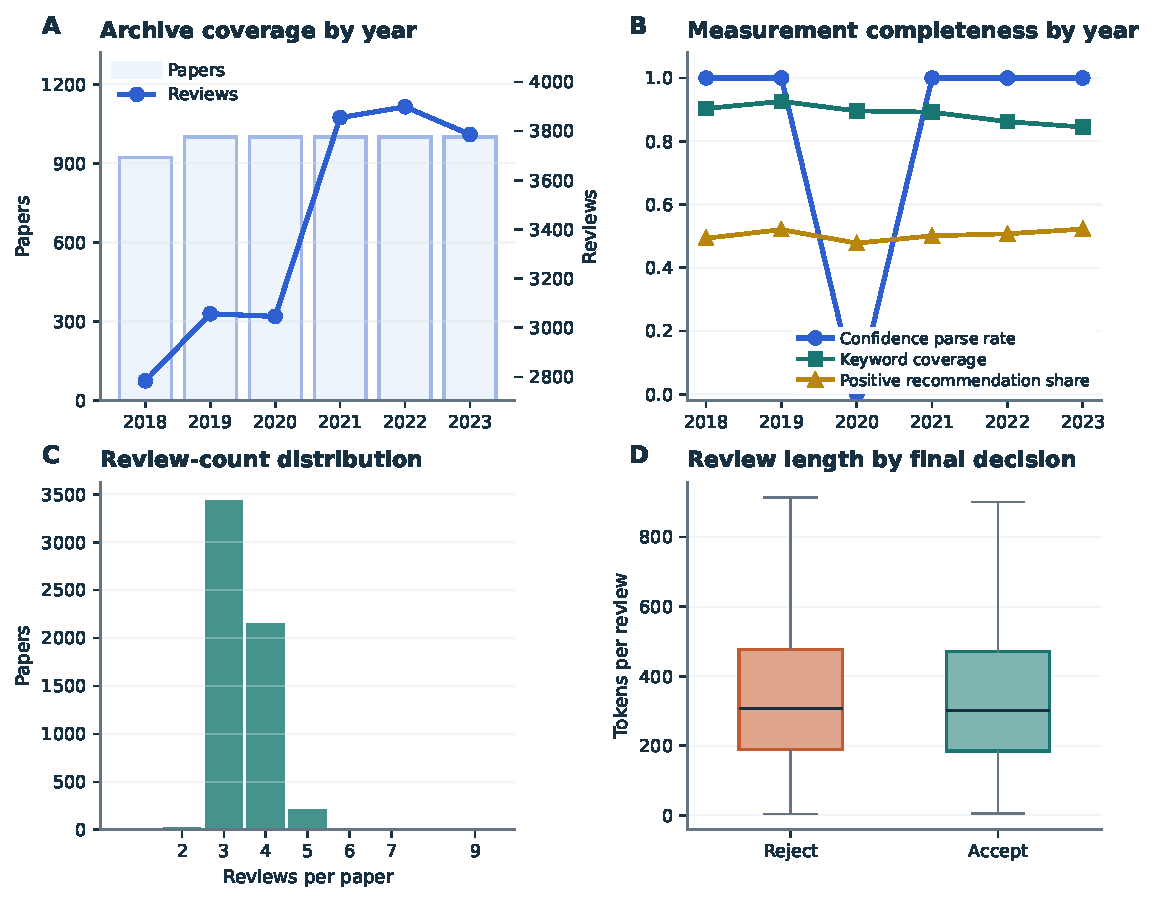
\includegraphics[width=0.98\linewidth]{appendix_figure_measurement_summary.pdf}
\caption{Measurement and archive-validation diagnostics. \textbf{A}, yearly paper and review counts in the harmonized archive. \textbf{B}, confidence parsing, keyword coverage, and positive-review prevalence by year; the clearest discontinuity is the loss of comparable confidence parsing in 2020. \textbf{C}, the distribution of reviews per paper, showing that the archive is concentrated around three to four reviews per submission. \textbf{D}, review-length distributions by final decision. Taken together, these panels document the scale of the archive and the practical boundaries of the measurement layer before any modeling begins.}
\label{fig:app:measurement}
\end{figure}

\begin{figure}[!htbp]
\centering
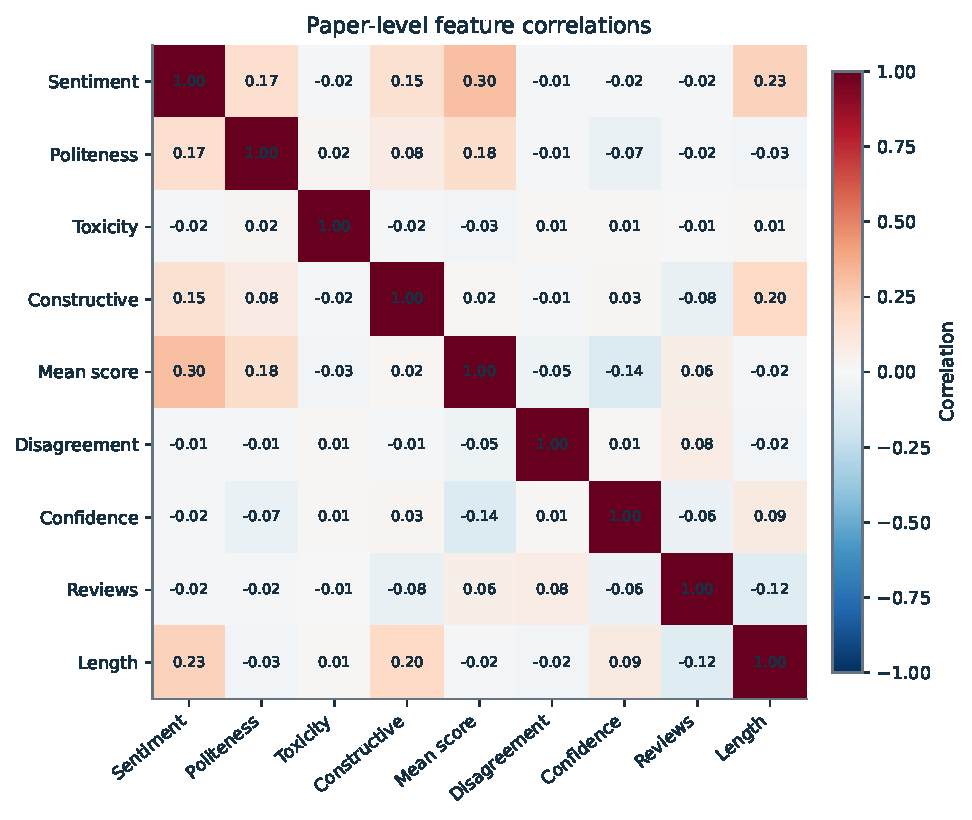
\includegraphics[width=0.98\linewidth]{appendix_figure_feature_correlations.pdf}
\caption{Paper-level correlation structure for language measures, score proxies, and review-structure covariates. The matrix shows that sentiment co-moves with reviewer score and, more modestly, with review length, whereas toxicity is only weakly related to most other observables. This matters for interpretation: the language measures do not float outside the rest of the evaluation record, but are embedded in the same broader profile that also contains scores, confidence, and review structure.}
\label{fig:app:correlations}
\end{figure}

\begin{table}[!htbp]
\centering
\begingroup
\scriptsize
\renewcommand{\arraystretch}{1.20}
\setlength{\tabcolsep}{6pt}
\caption{Raw-archive parsing diagnostics by year. The builder retains raw strings, parsed numeric fields, and parse-success flags for ratings, confidence, and final decisions. The table makes visible that parsing succeeds nearly completely for ratings and decisions across all years, while confidence is the one clear year-specific discontinuity because the 2020 raw export does not preserve a comparable confidence field.}
\label{tab:app:harmonization}
\begin{tabular}{rrrrrrrr}
\toprule
Year & Submissions & Reviews & Final decisions & Acceptance rate & Score parse rate & Confidence parse rate & Decision parse rate \\
\midrule
2018 & 935 & 2784 & 923 & 0.366 & 1.000 & 1.000 & 1.000 \\
2019 & 1000 & 3057 & 1000 & 0.391 & 1.000 & 1.000 & 1.000 \\
2020 & 1000 & 3046 & 1000 & 0.313 & 1.000 & 0.000 & 1.000 \\
2021 & 1000 & 3855 & 1000 & 0.316 & 1.000 & 1.000 & 1.000 \\
2022 & 1000 & 3899 & 1000 & 0.395 & 1.000 & 1.000 & 1.000 \\
2023 & 1000 & 3786 & 1000 & 0.407 & 1.000 & 1.000 & 1.000 \\
\bottomrule
\end{tabular}
\endgroup
\end{table}

\begin{table}[!htbp]
\centering
\begingroup
\normalsize
\renewcommand{\arraystretch}{1.20}
\setlength{\tabcolsep}{6pt}
\caption{Year-specific score and review-text sources used in the harmonized raw-archive parser. The table documents the exact field substitutions needed to make the archive comparable across years, especially the shift from \texttt{rating} to \texttt{recommendation} and the richer multi-field review text available in 2022--2023.}
\label{tab:app:fieldmap}
\begin{tabular}{rll}
\toprule
Year & Score field & Review-text field \\
\midrule
2018 & Rating & Review text \\
2019 & Rating & Review text \\
2020 & Rating & Review text \\
2021 & Rating & Review text \\
2022 & Recommendation & Paper summary + review summary \\
2023 & Recommendation & Paper summary + strengths and weaknesses + review summary \\
\bottomrule
\end{tabular}
\endgroup
\end{table}

\begin{table}[!htbp]
\centering
\begingroup
\scriptsize
\renewcommand{\arraystretch}{1.20}
\setlength{\tabcolsep}{6pt}
\caption{Measurement summary by year. The table reports archive scale, positive recommendation prevalence, parser completeness, manuscript-metadata missingness, and average review length. It shows that the reconstructed archive is large and fairly balanced across years, while also making clear that 2022 uses shorter review-text fields on average and that keyword coverage is imperfect but broadly usable for topic-proxy construction.}
\label{tab:app:measurementyear}
\resizebox{\textwidth}{!}{%
\begin{tabular}{rrrrrrrr}
\toprule
Year & Submissions & Reviews & Acceptance rate & Positive recommendation share & Confidence parse rate & Keyword missingness & Mean review length (tokens) \\
\midrule
2018 & 922 & 2784 & 0.366 & 0.493 & 1.000 & 0.097 & 369.843 \\
2019 & 1000 & 3057 & 0.391 & 0.520 & 1.000 & 0.074 & 405.720 \\
2020 & 1000 & 3046 & 0.313 & 0.478 & 0.000 & 0.104 & 412.030 \\
2021 & 1000 & 3855 & 0.316 & 0.501 & 1.000 & 0.108 & 478.825 \\
2022 & 1000 & 3899 & 0.395 & 0.507 & 1.000 & 0.138 & 147.583 \\
2023 & 1000 & 3786 & 0.407 & 0.522 & 1.000 & 0.155 & 398.375 \\
\bottomrule
\end{tabular}
}
\endgroup
\end{table}

\begin{table}[!htbp]
\centering
\begingroup
\normalsize
\renewcommand{\arraystretch}{1.20}
\setlength{\tabcolsep}{6pt}
\caption{Legacy lexicon inventory from the earlier exploratory workflow. These resources are preserved as measurement diagnostics rather than as the manuscript's source of truth. Including them here clarifies what the current rebuild inherited, checked, and simplified when moving from the older exploratory pipeline to the present raw-archive package.}
\label{tab:app:lexicon}
\begin{tabular}{lr}
\toprule
Lexicon & Entries \\
\midrule
Positive sentiment markers & 2449 \\
Negative sentiment markers & 5504 \\
AFINN sentiment scores & 2462 \\
Positive politeness markers & 95 \\
Negative politeness markers & 11 \\
Positive politeness phrases & 48 \\
Negative politeness phrases & 0 \\
Toxicity words & 5905 \\
Toxicity phrases & 1141 \\
Constructive feedback markers & 17 \\
Constructive feedback phrases & 31 \\
Hedging words & 41 \\
Hedging phrases & 16 \\
\bottomrule
\end{tabular}
\endgroup
\end{table}

\FloatBarrier
\vspace{0.6em}
\section*{Appendix: Bridge and Observational Diagnostics}
The next set of appendix materials expands the observational story by showing how descriptive language gaps behave inside score bins and how the paper-level sentiment association varies across topic-cluster proxies.

\begin{figure}[!htbp]
\centering
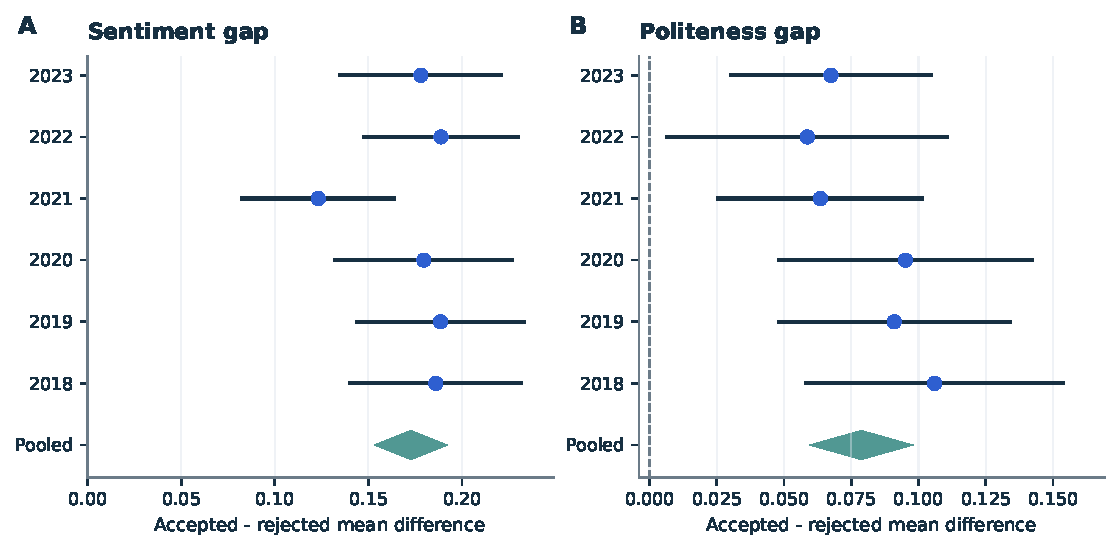
\includegraphics[width=0.98\linewidth]{figure3_temporal_stability.pdf}
\caption{Temporal stability of the descriptive language gap. Accepted-minus-rejected differences are shown separately for sentiment and politeness in each conference year, with pooled summaries shown below the year-specific estimates. The direction of the gap does not reverse in any year for either measure, which is why the main text describes this descriptive pattern as the most stable regularity in the paper.}
\label{fig:app:temporal}
\end{figure}

\begin{figure}[!htbp]
\centering
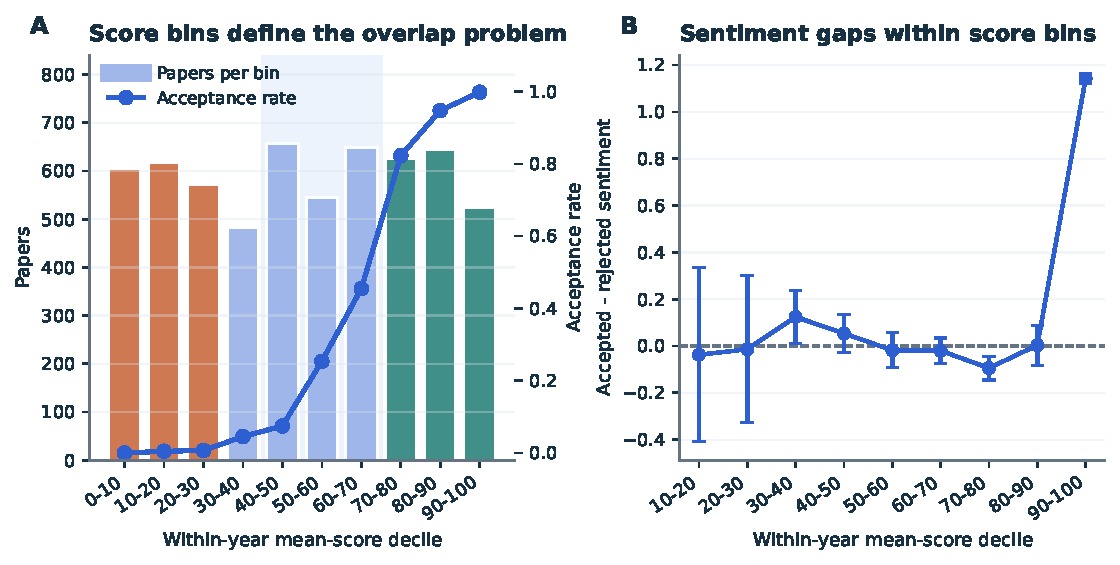
\includegraphics[width=0.98\linewidth]{appendix_figure_score_bridge.pdf}
\caption{Bridge analysis linking the full-sample descriptive layer to the matched borderline layer. \textbf{A}, acceptance rates across within-year mean-score deciles, with bar color tracking the decision mix of each bin. \textbf{B}, accepted-minus-rejected sentiment gaps within the same score bins. The key pattern is attenuation in the middle of the score distribution, where accepted and rejected papers overlap most plausibly; by contrast, the largest raw differences occur in regions where decisions are already nearly deterministic.}
\label{fig:app:bridge}
\end{figure}

\begin{figure}[!htbp]
\centering
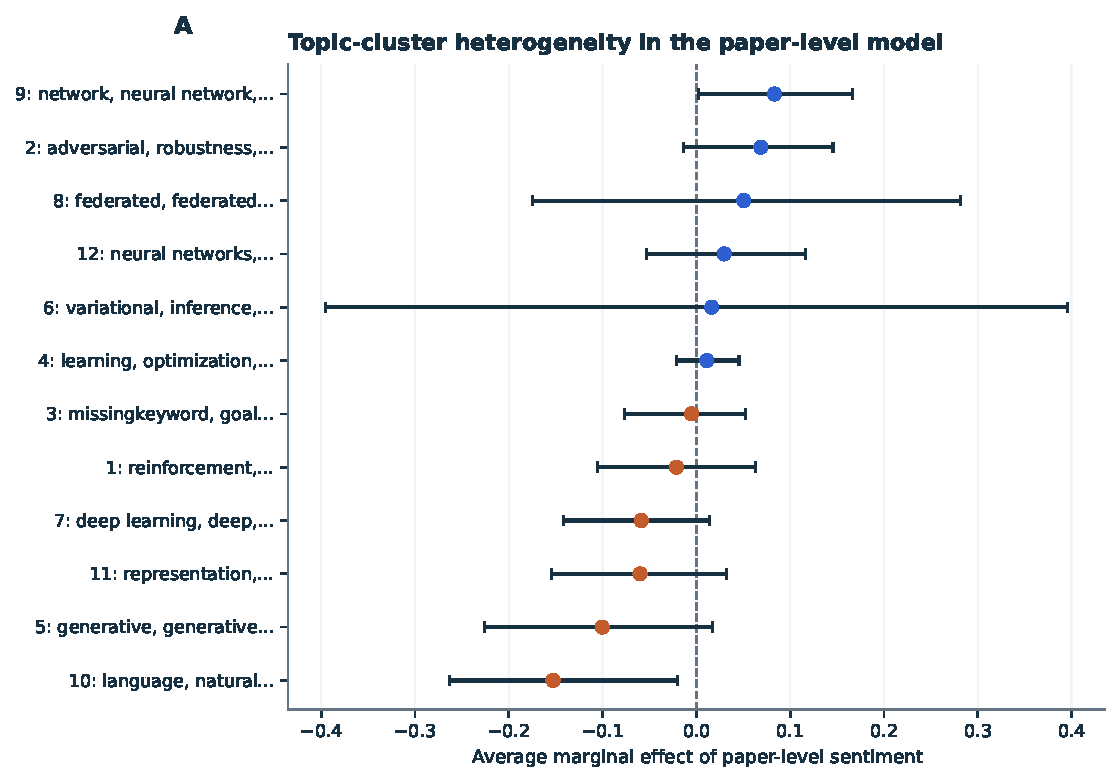
\includegraphics[width=0.98\linewidth]{appendix_figure_topic_heterogeneity.pdf}
\caption{Topic-cluster heterogeneity in the paper-level sentiment association. Topic controls are keyword-based clusters and should be interpreted as noisy topical proxies rather than official research areas. Most topic-specific estimates are imprecise and none reveals an obvious subfield in which the conditional paper-level sentiment association becomes consistently large and positive.}
\label{fig:app:topichetero}
\end{figure}

\begin{table}[!htbp]
\centering
\begingroup
\normalsize
\renewcommand{\arraystretch}{1.20}
\setlength{\tabcolsep}{6pt}
\caption{Average marginal effects from the paper-level fixed-effects model. The outcome is final acceptance. Full models include the broader score, disagreement, confidence, review-structure, manuscript-side, year, and topic controls described in the main text; this table isolates the language dimensions because they are central to the paper's substantive argument.}
\label{tab:app:paperame}
\begin{tabular}{lrrr}
\toprule
Predictor & Average marginal effect & 95\% CI lower & 95\% CI upper \\
\midrule
Paper-level mean review sentiment & -0.002 & -0.017 & 0.014 \\
Paper-level mean review politeness & -0.011 & -0.024 & 0.003 \\
Paper-level mean review toxicity & 0.750 & -0.568 & 2.209 \\
Paper-level mean review constructiveness & -0.009 & -0.020 & 0.003 \\
Mean reviewer score & 0.262 & 0.254 & 0.270 \\
Reviewer score disagreement & 0.003 & -0.005 & 0.012 \\
Mean reviewer confidence & -0.002 & -0.021 & 0.018 \\
Number of reviews & -0.005 & -0.030 & 0.022 \\
Mean review length (tokens) & -0.000 & -0.000 & 0.000 \\
Title length (tokens) & -0.001 & -0.003 & 0.000 \\
Abstract length (tokens) & -0.000 & -0.000 & 0.000 \\
Number of keywords & 0.004 & 0.000 & 0.007 \\
\bottomrule
\end{tabular}
\endgroup
\end{table}

\begin{table}[!htbp]
\centering
\begingroup
\normalsize
\renewcommand{\arraystretch}{1.20}
\setlength{\tabcolsep}{6pt}
\caption{Average marginal effects from the review-level fixed-effects model. The outcome is a positive reviewer recommendation (rating or recommendation score $\ge 6$). As in the main text, the table highlights that review-level sentiment has a much larger association with recommendation than any other tone dimension, which is why the review-level model is treated as the clearest evidence that language tracks reviewer stance.}
\label{tab:app:reviewame}
\begin{tabular}{lrrr}
\toprule
Predictor & Average marginal effect & 95\% CI lower & 95\% CI upper \\
\midrule
Review sentiment & 0.195 & 0.181 & 0.211 \\
Review politeness & 0.048 & 0.036 & 0.059 \\
Review toxicity & -0.376 & -0.768 & 0.063 \\
Review constructiveness & 0.011 & 0.002 & 0.018 \\
Reviewer confidence & -0.079 & -0.089 & -0.069 \\
Confidence missingness indicator & 0.004 & -0.136 & 0.153 \\
Review length (tokens) & -0.000 & -0.000 & -0.000 \\
Title length (tokens) & -0.004 & -0.007 & -0.001 \\
Abstract length (tokens) & 0.000 & -0.000 & 0.000 \\
Number of keywords & 0.002 & -0.002 & 0.008 \\
\bottomrule
\end{tabular}
\endgroup
\end{table}

\begin{table}[!htbp]
\centering
\begingroup
\normalsize
\renewcommand{\arraystretch}{1.20}
\setlength{\tabcolsep}{6pt}
\caption{Accepted-minus-rejected yearly descriptive gaps for the two main language dimensions discussed in the paper. Sentiment differences are positive in every year and larger than politeness differences throughout, reinforcing the interpretation that evaluative valence rather than generic civility is doing most of the descriptive work.}
\label{tab:app:yearlygaps}
\begin{tabular}{lrrrr}
\toprule
Language dimension & Year & Mean difference & 95\% CI lower & 95\% CI upper \\
\midrule
Sentiment gap & 2018 & 0.186 & 0.139 & 0.233 \\
Sentiment gap & 2019 & 0.189 & 0.143 & 0.234 \\
Sentiment gap & 2020 & 0.180 & 0.132 & 0.228 \\
Sentiment gap & 2021 & 0.123 & 0.082 & 0.165 \\
Sentiment gap & 2022 & 0.189 & 0.147 & 0.231 \\
Sentiment gap & 2023 & 0.178 & 0.134 & 0.222 \\
Politeness gap & 2018 & 0.106 & 0.058 & 0.154 \\
Politeness gap & 2019 & 0.091 & 0.047 & 0.135 \\
Politeness gap & 2020 & 0.095 & 0.048 & 0.143 \\
Politeness gap & 2021 & 0.064 & 0.025 & 0.102 \\
Politeness gap & 2022 & 0.059 & 0.006 & 0.111 \\
Politeness gap & 2023 & 0.067 & 0.030 & 0.105 \\
\bottomrule
\end{tabular}
\endgroup
\end{table}

\begin{table}[!htbp]
\centering
\begingroup
\scriptsize
\renewcommand{\arraystretch}{1.20}
\setlength{\tabcolsep}{6pt}
\caption{Within-score-bin bridge diagnostics. Bins are based on the within-year percentile of paper-level mean score. This table underlies the bridge figure and shows numerically that the accepted-minus-rejected sentiment gap is much smaller in the central score bins than in the extreme bins where acceptance is nearly certain or nearly impossible.}
\label{tab:app:bridge}
\resizebox{\textwidth}{!}{%
\begin{tabular}{lrrrrrrr}
\toprule
Score decile & Submissions & Accepted submissions & Rejected submissions & Acceptance rate & Sentiment difference & 95\% CI lower & 95\% CI upper \\
\midrule
0-10 & 605 & 0 & 605 & 0.000 & NA & NA & NA \\
10-20 & 618 & 3 & 615 & 0.005 & -0.038 & -0.410 & 0.334 \\
20-30 & 573 & 4 & 569 & 0.007 & -0.014 & -0.329 & 0.301 \\
30-40 & 483 & 22 & 461 & 0.046 & 0.124 & 0.010 & 0.238 \\
40-50 & 656 & 49 & 607 & 0.075 & 0.054 & -0.027 & 0.135 \\
50-60 & 544 & 138 & 406 & 0.254 & -0.018 & -0.093 & 0.057 \\
60-70 & 649 & 295 & 354 & 0.455 & -0.020 & -0.075 & 0.034 \\
70-80 & 625 & 514 & 111 & 0.822 & -0.094 & -0.145 & -0.043 \\
80-90 & 645 & 611 & 34 & 0.947 & 0.003 & -0.082 & 0.089 \\
90-100 & 524 & 523 & 1 & 0.998 & 1.142 & 1.122 & 1.163 \\
\bottomrule
\end{tabular}
}
\endgroup
\end{table}

\begin{table}[!htbp]
\centering
\begingroup
\small
\renewcommand{\arraystretch}{1.20}
\setlength{\tabcolsep}{6pt}
\caption{Year-specific average marginal effects of paper-level sentiment in the paper-level model. The estimates move around zero but do not reveal a year in which the conditional paper-level sentiment association becomes both large and precisely positive.}
\label{tab:app:heteroyear}
\begin{tabular}{rrrrl}
\toprule
Year & Average marginal effect & 95\% CI lower & 95\% CI upper & Specification note \\
\midrule
2018 & 0.015 & -0.044 & 0.073 & Requested specification \\
2019 & 0.005 & -0.046 & 0.052 & Requested specification \\
2020 & -0.039 & -0.039 & -0.039 & Requested specification \\
2021 & 0.024 & -0.030 & 0.074 & Requested specification \\
2022 & 0.009 & -0.050 & 0.067 & Requested specification \\
2023 & -0.022 & -0.075 & 0.029 & Requested specification \\
\bottomrule
\end{tabular}
\endgroup
\end{table}

\begin{table}[!htbp]
\centering
\begingroup
\normalsize
\renewcommand{\arraystretch}{1.20}
\setlength{\tabcolsep}{6pt}
\caption{Average marginal effects of paper-level sentiment by disagreement tercile. This table complements the main heterogeneity figure by showing numerically that high reviewer disagreement does not produce a markedly larger positive paper-level sentiment effect.}
\label{tab:app:heterodisagreement}
\begin{tabular}{lrrrl}
\toprule
Reviewer disagreement tier & Average marginal effect & 95\% CI lower & 95\% CI upper & Specification note \\
\midrule
Low disagreement & -0.021 & -0.059 & 0.012 & HC1 covariance fallback \\
Medium disagreement & 0.008 & -0.027 & 0.043 & Requested specification \\
High disagreement & 0.006 & -0.038 & 0.052 & HC1 covariance fallback \\
\bottomrule
\end{tabular}
\endgroup
\end{table}

\begin{table}[!htbp]
\centering
\begingroup
\normalsize
\renewcommand{\arraystretch}{1.20}
\setlength{\tabcolsep}{6pt}
\caption{Average marginal effects of paper-level sentiment by keyword-based topic cluster. Because the topic clusters are deterministic keyword proxies rather than official tracks, the table is best read as a boundary check: it helps rule out the concern that the pooled near-null paper-level estimate is hiding one dominant topic-specific positive effect.}
\label{tab:app:heterotopic}
\begin{tabular}{rrrrrl}
\toprule
Topic cluster & Submissions & Average marginal effect & 95\% CI lower & 95\% CI upper & Representative keywords \\
\midrule
1 & 641 & -0.021 & -0.106 & 0.063 & reinforcement, reinforcement... \\
2 & 224 & 0.069 & -0.014 & 0.146 & adversarial, robustness, examples,... \\
3 & 668 & -0.005 & -0.077 & 0.052 & missingkeyword, goal conditioned,... \\
4 & 2275 & 0.011 & -0.021 & 0.045 & learning, optimization, model,... \\
5 & 289 & -0.100 & -0.226 & 0.017 & generative, generative models,... \\
6 & 120 & 0.016 & -0.396 & 0.396 & variational, inference, variational... \\
7 & 476 & -0.059 & -0.142 & 0.014 & deep learning, deep, learning,... \\
8 & 78 & 0.050 & -0.175 & 0.282 & federated, federated learning,... \\
9 & 263 & 0.083 & 0.002 & 0.166 & network, neural network, neural,... \\
10 & 155 & -0.153 & -0.263 & -0.020 & language, natural language,... \\
11 & 274 & -0.060 & -0.155 & 0.032 & representation, representation... \\
12 & 459 & 0.030 & -0.053 & 0.117 & neural networks, networks, neural,... \\
\bottomrule
\end{tabular}
\endgroup
\end{table}

\begin{figure}[!htbp]
\centering
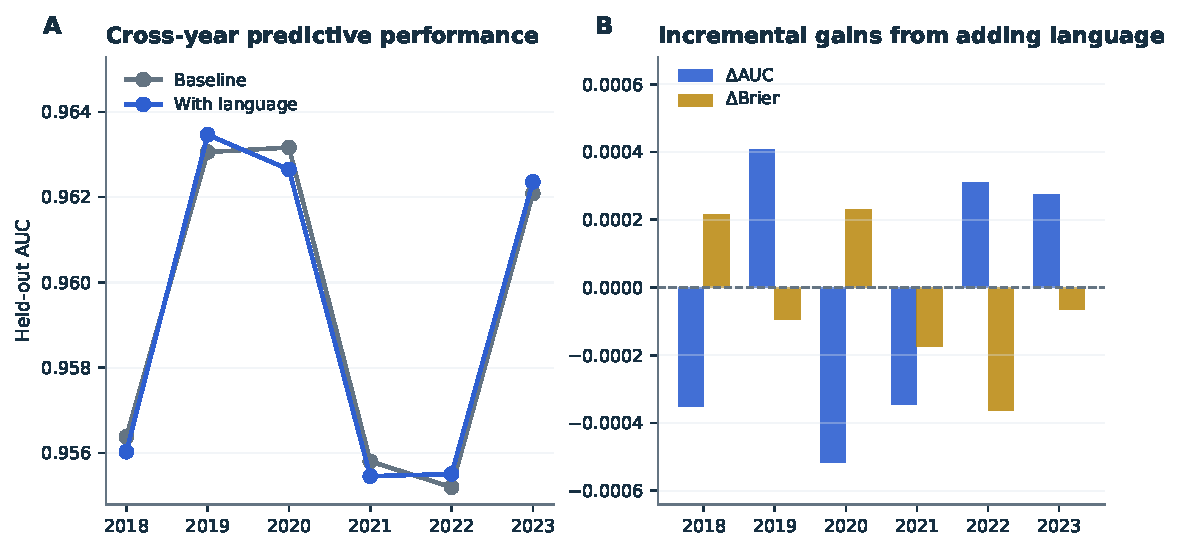
\includegraphics[width=0.98\linewidth]{appendix_figure_prediction_diagnostics.pdf}
\caption{Appendix-only predictive diagnostics. \textbf{A}, held-out AUC for the baseline model and the model augmented with paper-level language features. \textbf{B}, incremental gains from adding language on held-out AUC and Brier score by year. Held-out discrimination is already high in the score-based baseline models, and the incremental changes from adding language are tiny in absolute magnitude, which is why prediction is treated as a boundary condition rather than as a headline contribution.}
\label{fig:app:prediction}
\end{figure}

\begin{table}[!htbp]
\centering
\begingroup
\normalsize
\renewcommand{\arraystretch}{1.20}
\setlength{\tabcolsep}{6pt}
\caption{Appendix-only leave-one-year-out predictive diagnostics. The baseline uses score and manuscript controls; the extended model adds paper-level language features. Held-out AUC is already high in the baseline models, and the incremental changes from adding language are extremely small in absolute magnitude, which is why prediction is treated as a boundary condition rather than as a headline contribution.}
\label{tab:app:prediction}
\begin{tabular}{rrrrrr}
\toprule
Held-out year & Baseline AUC & AUC with language & AUC change & Log-loss change & Brier-score change \\
\midrule
2018 & 0.956 & 0.956 & -0.000 & 0.000 & 0.000 \\
2019 & 0.963 & 0.963 & 0.000 & -0.001 & -0.000 \\
2020 & 0.963 & 0.963 & -0.001 & 0.002 & 0.000 \\
2021 & 0.956 & 0.955 & -0.000 & -0.001 & -0.000 \\
2022 & 0.955 & 0.956 & 0.000 & -0.001 & -0.000 \\
2023 & 0.962 & 0.962 & 0.000 & -0.000 & -0.000 \\
\bottomrule
\end{tabular}
\endgroup
\end{table}

\FloatBarrier
\vspace{0.6em}
\section*{Appendix: Matched Observational Diagnostics}
These appendix materials document overlap, balance, and sample composition for the matched borderline design and its sensitivities.

\begin{figure}[!htbp]
\centering
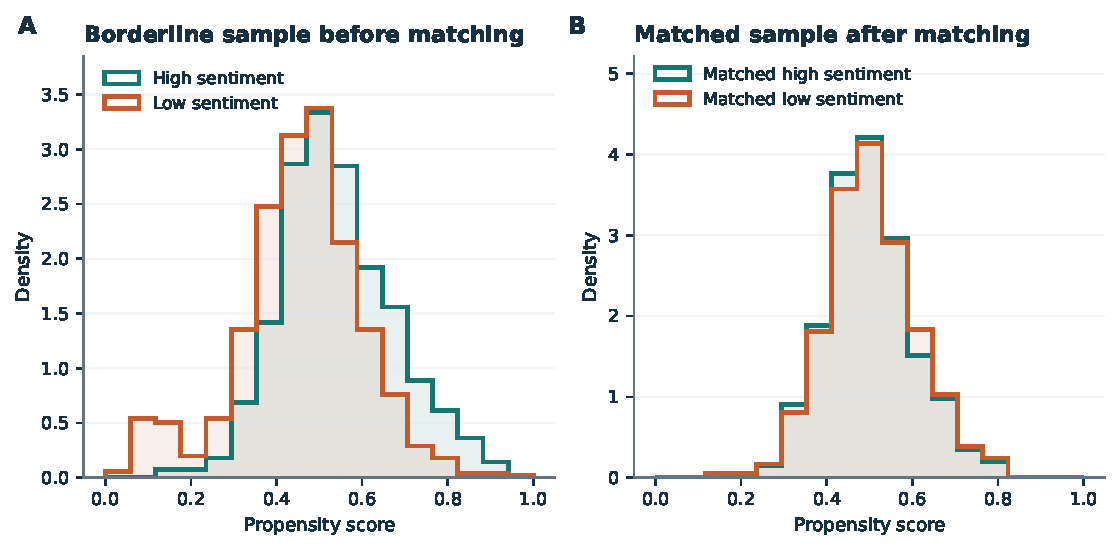
\includegraphics[width=0.98\linewidth]{appendix_figure_psm_overlap.pdf}
\caption{Propensity-score overlap for the primary borderline specification before and after matching. The matched sample retains substantial overlap while sharpening comparability between the higher-sentiment and lower-sentiment groups. This diagnostic matters because it shows that the near-zero matched estimate is not being produced by an obviously broken common-support region.}
\label{fig:app:overlap}
\end{figure}

\begin{table}[!htbp]
\centering
\begingroup
\small
\renewcommand{\arraystretch}{1.20}
\setlength{\tabcolsep}{6pt}
\caption{Matched observational evidence from the borderline layer. The table reports the primary 35th-65th percentile window, two prespecified window sensitivities, and the top-versus-bottom sentiment-tercile sensitivity check. Across all four designs, estimated sentiment-linked differences in acceptance remain modest and their confidence intervals include differences close to zero, which is why the matched layer is interpreted as conservative validation rather than as the paper's strongest positive result.}
\label{tab:app:matchingeffects}
\begin{tabular}{lrrrrr}
\toprule
Matching specification & Matched contrast (ATT) & 95\% CI lower & 95\% CI upper & Matched pairs & Balance target met \\
\midrule
Primary 35-65 window & 0.004 & -0.037 & 0.043 & 695 & Yes \\
Window 40-60 & 0.009 & -0.040 & 0.054 & 429 & Yes \\
Window 30-70 & 0.011 & -0.027 & 0.052 & 850 & Yes \\
Top vs bottom terciles & -0.054 & -0.109 & 0.000 & 404 & Yes \\
\bottomrule
\end{tabular}
\endgroup
\end{table}

\begin{table}[!htbp]
\centering
\begingroup
\normalsize
\renewcommand{\arraystretch}{1.20}
\setlength{\tabcolsep}{6pt}
\caption{Standardized mean differences before and after matching for the primary borderline matched sample. The core balance target is $|SMD| < 0.10$ after matching. The table shows that the largest pre-match imbalance is in mean review length and that this imbalance contracts sharply after matching along with the smaller imbalances in score, disagreement, confidence, and manuscript-side covariates.}
\label{tab:app:balance}
\begin{tabular}{lrr}
\toprule
Covariate & Absolute SMD before matching & Absolute SMD after matching \\
\midrule
Mean reviewer score & 0.030 & 0.009 \\
Reviewer score disagreement & -0.072 & -0.007 \\
Mean reviewer confidence & 0.093 & -0.023 \\
Number of reviews & -0.011 & 0.012 \\
Mean review length (tokens) & 0.339 & -0.016 \\
Title length (tokens) & -0.022 & -0.021 \\
Abstract length (tokens) & -0.006 & 0.007 \\
Number of keywords & -0.003 & 0.011 \\
\bottomrule
\end{tabular}
\endgroup
\end{table}

\begin{table}[!htbp]
\centering
\begingroup
\scriptsize
\renewcommand{\arraystretch}{1.20}
\setlength{\tabcolsep}{6pt}
\caption{Overlap summaries for the primary and sensitivity matched designs. The table reports the size of the analytic samples, the extent of common support, and the caliper used in each specification so that the reader can evaluate how much overlap is retained as the design window narrows or widens.}
\label{tab:app:overlap}
\resizebox{\textwidth}{!}{%
\begin{tabular}{lrrrrrrrl}
\toprule
Matching specification & Analytic sample size & Higher-sentiment papers & Lower-sentiment papers & Matched pairs & Common-support lower bound & Common-support upper bound & Caliper & Balance target met \\
\midrule
Primary 35-65 window & 1878 & 937 & 941 & 695 & 0.119 & 0.942 & 0.069 & Yes \\
Window 40-60 & 1200 & 598 & 602 & 429 & 0.169 & 0.941 & 0.065 & Yes \\
Window 30-70 & 2332 & 1164 & 1168 & 850 & 0.094 & 0.931 & 0.071 & Yes \\
Top vs bottom terciles & 1256 & 631 & 625 & 404 & 0.085 & 0.931 & 0.099 & Yes \\
\bottomrule
\end{tabular}
}
\endgroup
\end{table}

\begin{table}[!htbp]
\centering
\begingroup
\normalsize
\renewcommand{\arraystretch}{1.20}
\setlength{\tabcolsep}{6pt}
\caption{Matched-pair counts by year for the primary borderline specification. The matched sample is distributed across all six conference years, indicating that the primary matched design is not driven by one unusually well-behaved cohort.}
\label{tab:app:matchedcounts}
\begin{tabular}{rr}
\toprule
Year & Matched pairs \\
\midrule
2018 & 99 \\
2019 & 105 \\
2020 & 123 \\
2021 & 97 \\
2022 & 138 \\
2023 & 133 \\
\bottomrule
\end{tabular}
\endgroup
\end{table}

\begin{table}[!htbp]
\centering
\begingroup
\normalsize
\renewcommand{\arraystretch}{1.20}
\setlength{\tabcolsep}{6pt}
\caption{Deterministic keyword-based topic clusters used as topic fixed effects in the main models. The table is included for transparency because the paper does not claim official area-level stability; instead, these clusters serve as reproducible but noisy controls for topical composition.}
\label{tab:app:topics}
\begin{tabular}{rrl}
\toprule
Topic cluster & Submissions & Representative keywords \\
\midrule
1 & 641 & reinforcement, reinforcement... \\
2 & 224 & adversarial, robustness, examples,... \\
3 & 668 & missingkeyword, goal conditioned,... \\
4 & 2276 & learning, optimization, model,... \\
5 & 289 & generative, generative models,... \\
6 & 120 & variational, inference, variational... \\
7 & 476 & deep learning, deep, learning,... \\
8 & 78 & federated, federated learning,... \\
9 & 263 & network, neural network, neural,... \\
10 & 155 & language, natural language,... \\
11 & 274 & representation, representation... \\
12 & 459 & neural networks, networks, neural,... \\
\bottomrule
\end{tabular}
\endgroup
\end{table}

\FloatBarrier
\vspace{0.6em}
\section*{Appendix: Legacy Diagnostics from Earlier Derived Tables}
The final appendix section preserves selected outputs from the earlier exploratory derived-table workflow. These materials remain useful as exploratory diagnostics and figure prototypes, but they are not the manuscript's primary evidentiary base.

\begin{figure}[!htbp]
\centering
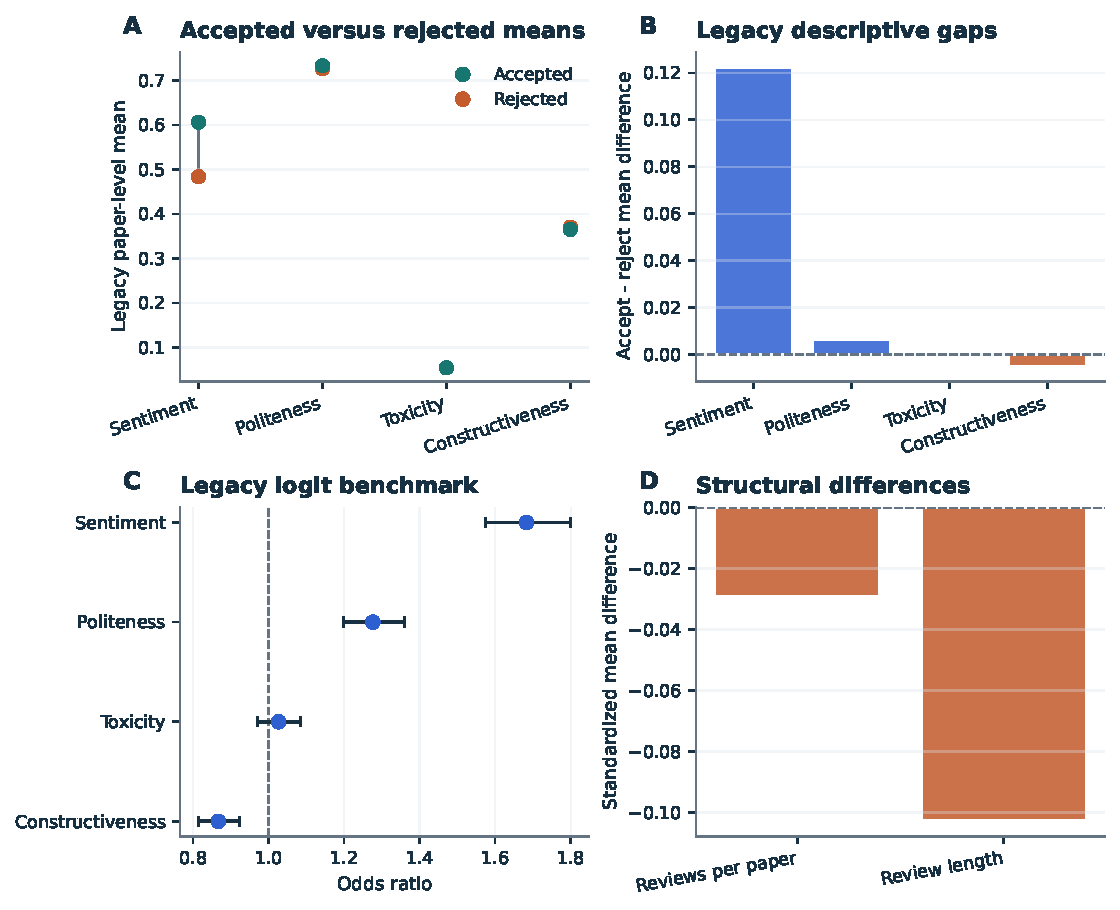
\includegraphics[width=0.98\linewidth]{appendix_figure_legacy_rq1.pdf}
\caption{Legacy descriptive diagnostics from the earlier derived-table workflow, redrawn here in a cleaner format and retained as exploratory benchmarks for the expanded raw-archive rebuild. Their role is historical rather than inferential: they show that the archive-first package preserves the broad descriptive story while improving traceability and measurement transparency.}
\label{fig:app:legacyrq1}
\end{figure}

\begin{figure}[!htbp]
\centering
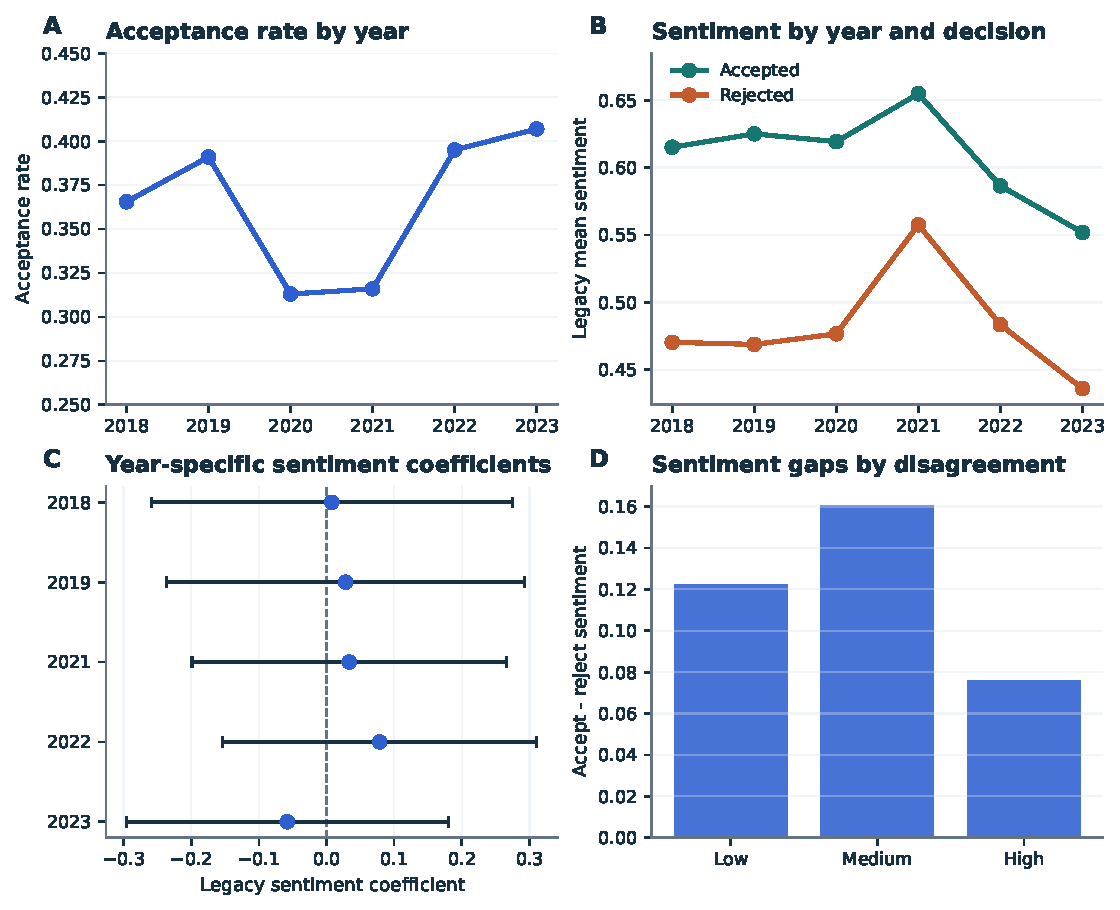
\includegraphics[width=0.98\linewidth]{appendix_figure_legacy_rq3.pdf}
\caption{Legacy temporal and subgroup diagnostics from the earlier derived-table workflow, retained as appendix-only materials for comparison with the current archive-first analysis. Their role is archival rather than evidentiary: they show how the present manuscript reorganizes earlier stability patterns into a broader and more auditable design.}
\label{fig:app:legacyrq3}
\end{figure}

\begin{table}[!htbp]
\centering
\begingroup
\small
\renewcommand{\arraystretch}{1.20}
\setlength{\tabcolsep}{6pt}
\caption{Legacy multivariable logit benchmark from the earlier derived-table workflow. This table is retained only as a benchmark against the previous pipeline and should not be treated as the manuscript's primary source of inference.}
\label{tab:app:legacymultivariable}
\begin{tabular}{lrrrr}
\toprule
Predictor & Odds ratio & 95\% CI lower & 95\% CI upper & P-value \\
\midrule
Legacy sentiment & 1.683 & 1.574 & 1.799 & 0.000 \\
Legacy politeness & 1.276 & 1.198 & 1.359 & 0.000 \\
Legacy toxicity & 1.026 & 0.972 & 1.084 & 0.350 \\
Legacy constructiveness & 0.867 & 0.815 & 0.922 & 0.000 \\
Legacy reviews per paper & 0.953 & 0.902 & 1.007 & 0.090 \\
Legacy review length & 0.795 & 0.749 & 0.844 & 0.000 \\
\bottomrule
\end{tabular}
\endgroup
\end{table}

\begin{table}[!htbp]
\centering
\begingroup
\normalsize
\renewcommand{\arraystretch}{1.20}
\setlength{\tabcolsep}{6pt}
\caption{Legacy stability summary from the earlier exploratory workflow. As with the previous legacy table, this summary is included to document continuity with the exploratory stage of the project rather than to substitute for the raw-archive analyses reported in the main text and earlier appendix sections.}
\label{tab:app:legacymeta}
\begin{tabular}{lrrl}
\toprule
Measure & Pooled effect & I-squared (\%) & Stability pattern \\
\midrule
Legacy sentiment & 0.019 & 0.000 & stable (low heterogeneity) \\
Legacy politeness & 0.089 & 0.000 & stable (low heterogeneity) \\
Legacy toxicity & 0.031 & 14.410 & stable (low heterogeneity) \\
Legacy constructiveness & -0.026 & 46.917 & partially stable (moderate heterogeneity) \\
\bottomrule
\end{tabular}
\endgroup
\end{table}



\end{document}
